\documentclass[12pt,a4paper,utf8x]{report}
\usepackage [english]{babel}

% Pour pouvoir utiliser 
\usepackage{ucs}
\usepackage[utf8x]{inputenc}

\usepackage{pifont}
\newcommand{\tick}{\ding{51}} % to write ticks
\newcommand{\badtick}{\ding{55}} % to write cross

\usepackage[pdftex]{graphicx} % to include pictures
\usepackage{pdfpages} % to include PDF pages as pictures (1st and last page)

\usepackage{url} % Pour avoir de belles url
\usepackage {geometry}

\usepackage{color}
\usepackage{xcolor}

% Pour mettre du code source
\usepackage {listings}
% Pour pouvoir passer en paysage
\usepackage{lscape}

\usepackage{caption}
\DeclareCaptionFont{white}{\color{white}}
\DeclareCaptionFormat{listing}{\colorbox{gray}{\parbox{\textwidth}{#1#2#3}}}
\captionsetup[lstlisting]{format=listing,labelfont=white,textfont=white}

\lstdefinelanguage{JavaScript}{
     keywords={attributes, class, classend, do, empty, endif, endwhile, fail, function, functionend, if, implements, in, inherit, inout, not, of, operations, out, return, set, then, types, while, use},
     keywordstyle=\color{blue}\bfseries,
     ndkeywords={},
     ndkeywordstyle=\color{yellow}\bfseries,
     identifierstyle=\color{black},
     sensitive=false,
     comment=[l]{//},
     commentstyle=\color{green}\ttfamily,
     stringstyle=\color{red}\ttfamily
  }

  \usepackage{courier}
 \lstset{
         basicstyle=\footnotesize\ttfamily, % Standardschrift
         %numbers=left,               % Ort der Zeilennummern
         numberstyle=\tiny,          % Stil der Zeilennummern
         %stepnumber=2,               % Abstand zwischen den Zeilennummern
         numbersep=5pt,              % Abstand der Nummern zum Text
         tabsize=2,                  % Groesse von Tabs
         extendedchars=true,         %
         breaklines=true,            % Zeilen werden Umgebrochen
         keywordstyle=\color{red},
    		frame=b,      	
    	 identifierstyle=\ttfamily,   
		 keywordstyle=\color[rgb]{0,0,1},
         commentstyle=\color[rgb]{0.133,0.545,0.133},
         stringstyle=\color[rgb]{0.627,0.126,0.941},
         %stringstyle=\color{white}\ttfamily, % Farbe der String
         showspaces=false,           % Leerzeichen anzeigen ?
         showtabs=false,             % Tabs anzeigen ?
         xleftmargin=17pt,
         framexleftmargin=17pt,
         framexrightmargin=5pt,
         framexbottommargin=4pt,
         %backgroundcolor=\color{lightgray},
         showstringspaces=false      % Leerzeichen in Strings anzeigen ?        
 }
 
 \lstloadlanguages{XML, HTML,Java,PHP,SQL,JavaScript}


% Pour pouvoir faire plusieurs colonnes
\usepackage {multicol}
% POur crééer un index
\usepackage{makeidx}
\makeindex

% Pour les entetes de page
\usepackage{fancyhdr} % Header and footnotes
\pagestyle{fancy}
\renewcommand{\chaptermark}[1]{\markboth{#1}{}}
\renewcommand{\sectionmark}[1]{\markright{\thesection\ #1}}
\fancyhf{} \fancyhead[LE,RO]{\bfseries\thepage}
\fancyhead[LO]{\bfseries\rightmark}
\fancyhead[RE]{\bfseries\leftmark}
\renewcommand{\headrulewidth}{0.5pt}
\addtolength{\headheight}{0.5pt}
\addtolength{\headwidth}{100pt }
\renewcommand{\footrulewidth}{0pt}

% Pour l'interligne de 1.5
\usepackage {setspace}
% Pour les marges de la page
\geometry{a4paper, top=2.5cm, bottom=3.5cm, left=1.5cm, right=1.5cm, marginparwidth=1.2cm}

\parskip=5pt %% distance entre § (paragraphe)
\sloppy %% respecter toujours la marge de droite 

% Pour les pénalités :
\interfootnotelinepenalty=150 %note de bas de page
\widowpenalty=150 %% veuves et orphelines
\clubpenalty=150 

%Pour la longueur de l'indentation des paragraphes
\setlength{\parindent}{15mm}



%%%% debut macro pour enlever le nom chapitre %%%%
\makeatletter
\def\@makechapterhead#1{%
  \vspace*{50\p@}%
  {\parindent \z@ \raggedright \normalfont
    \interlinepenalty\@M
    \ifnum \c@secnumdepth >\m@ne
        \Huge\bfseries \thechapter\quad
    \fi
    \Huge \bfseries #1\par\nobreak
    \vskip 40\p@
  }}

\def\@makeschapterhead#1{%
  \vspace*{50\p@}%
  {\parindent \z@ \raggedright
    \normalfont
    \interlinepenalty\@M
    \Huge \bfseries  #1\par\nobreak
    \vskip 40\p@
  }}
\makeatother
%%%% fin macro %%%%

%Couverture 
% Le plus simple est d'importer un pdf s'il y a une couverture type a respecter
%
\includepdf[pages=1,noautoscale=false]{premiere_page.pdf} 
\title
{
	\normalsize{DESS Xxxxx xxxx xxxxx\\
	Université de Xxxx Xxxxxx\\
	2004-2005}\\
	\vspace{15mm}
	\Huge{Titre du rapport de stage}
}
\author{Nom Auteur\\
	\vspace{45mm}
}

\date{	
	\normalsize{Lieu du stage\\
	Adresse du stage\\
	Ville du stage\\ 
	\vspace{5mm}	
	Directeur de recherche : M. DUPONT \\
	Rapporteur universitaire : Mme DUPUIS
	}
}

\begin{document}

\maketitle

\chapter*{Acknowledgements}
First I would like to thank Mr. TAEI Payman, Director of Operations and President of
Hindsite Interactive for allowing me to integrate this structure and have this unique
opportunity to realize my final degree project in the United States.
In particular I would like to thank Mr. TAEI for the confidence he granted to me to
lead the different projects I was affected to by considering me as an employee.
As my tutor I want to thank him for proposing me interesting, diversified and original
projects and tasks from a technical point of view. I especially enjoyed the autonomy
and responsibilities he entrusted me. But also follow-up, availability, advice and
criticism that enabled me to make progress and improve at the technical point of
view as well as methodological.
As well thank you to Mr. KHERADMAND Shayan, responsible of design who was
one of my co-worker and contact for all questions regarding the design. He was
always available and relevant in his answers.

I also would like to thank Mr. WEINZAPFEEL Pierre, ex-intern at Hindsite extending his
experience in the company for other six-months as a Web Developer. He was my
main co-worker and a precious help to understand the architecture and existing
code. Our mutual help allowed us to achieve a working project and a quick
progression of tasks.

Finally I thank all other employees of Hindsite at a distance or not for their patience
and help when needed.
%\clearpage

\tableofcontents
\listoffigures
\listoftables
\clearpage

% Pour avoir un interligne de 1,5
\begin{onehalfspace}

\chapter{Introduction}

During my last year of studies at the University of Technology of Belfort-
Montbeliard (UTBM) in Computer Science Engineering, I acquired the
theoretical fundamentals in computer engineering, more particularly in
Software and Knowledge Engineering. In order to achieve my master in
engineering degree, my curriculum requires a 24-weeks final degree project to
apply and develop my skills in a professional activity.

I have chosen to apply to do this internship at Hindsite Interactive in order to
go into details in the web development and multimedia fields of study, an area
in expansion that interests me more particularly. In addition I wanted to do this
project in a foreign country to continue my international experience initiated
with my ST40 (technical internship) in Basel, Switzerland. The project that
Hindsite offered me was ambitious and required the mastery of a range of
different technologies.

Hindsite Interactive is a small business specialized in multimedia, web
development, web design and website hosting. The main services proposed
are designing, web site creation and an online tool that can be compared to a
Content Management System (CMS) called Easy Web Content (EWC). This
tool allows customers to create a new website, edit an existing one and
manage their sites.

My internship as a junior web developer has for main task to create new add-
ons for EWC and to develop a manager to enable clients to create, customize,
edit and populate these add-ons. An add-on is defined as an interactive
dynamic module that can be embedded in their website by clients. The goal is
to realize a common structure for all add-ons to reduce development time for
further add-ons.

After a presentation of the company and the Easy Web Content site, I will
describe the organization of the internship and finally detail the achieved work.

\clearpage


%samples chapter
\chapter{Le titre du chapitre}

\section{Le titre de la section qui va bien}

\subsection{Titre de la sous section}

Exemple de code .
\lstset{language=HTML}
\begin{lstlisting}[label=some-css,caption=Some Html]
<style>
.header {
	background:#333;
	height:123px;

}
</style>

\end{lstlisting}
\lstset{language=PHP}
\begin{lstlisting}[label=some-php,caption=Some Php]
<?php
public class maClasse{
	public maFonction()
	{
		$maVar = new String("hello world");	
	}
}
?>

\end{lstlisting}
%$
\lstset{language=JavaScript}
\begin{lstlisting}[label=some-js,caption=Some JavaScript]

var mavar = new String('polop');
alert("hello world");
return false;

\end{lstlisting}

\lstset{language=SQL}
\begin{lstlisting}[label=some-sql,caption=Some SQL]

SELECT * FROM page WHERE id='1';

\end{lstlisting}

%-- Note de bas de page sur les stades
\protect\footnote{Par exemple, on peut faire un pied de page :
\begin{itemize}
\item avec une liste à puces ;
\item avec une liste à puces ;
\item avec une liste à puces.
\end{itemize}
}
%-- Fin Note de bas de page sur les stades

Ici du texte et du blabla, ce que l'on veut dire et écrire. A remplacer. Ici du texte et du blabla, ce que l'on veut dire et écrire. A remplacer. Ici du texte et du blabla, ce que l'on veut dire et écrire. A remplacer. Ici du texte et du blabla, ce que l'on veut dire et écrire. A remplacer. Ici du texte et du blabla, ce que l'on veut dire et écrire. A remplacer. Ici du texte et du blabla, ce que l'on veut dire et écrire. A remplacer.

\begin{itemize}
\item avec une liste à puces ;
\item avec une liste à puces ;
\item avec une liste à puces.
\end{itemize}

Ici du texte et du blabla, ce que l'on veut dire et écrire. A remplacer. Ici du texte et du blabla, ce que l'on veut dire et écrire. A remplacer. Ici du texte et du blabla, ce que l'on veut dire et écrire. A remplacer. Ici du texte et du blabla, ce que l'on veut dire et écrire. A remplacer. Ici du texte et du blabla, ce que l'on veut dire et écrire. A remplacer. Ici du texte et du blabla, ce que l'on veut dire et écrire. A remplacer.

\subsubsection{Titre de la sous sous section}

Ici du texte et du blabla, ce que l'on veut dire et écrire. A remplacer. Ici du texte et du blabla, ce que l'on veut dire et écrire. A remplacer. Ici du texte et du blabla, ce que l'on veut dire et écrire. A remplacer. Ici du texte et du blabla, ce que l'on veut dire et écrire. A remplacer. Ici du texte et du blabla, ce que l'on veut dire et écrire. A remplacer. Ici du texte et du blabla, ce que l'on veut dire et écrire. A remplacer.

%exemple d'image
\begin{figure}[!ht]
\centering
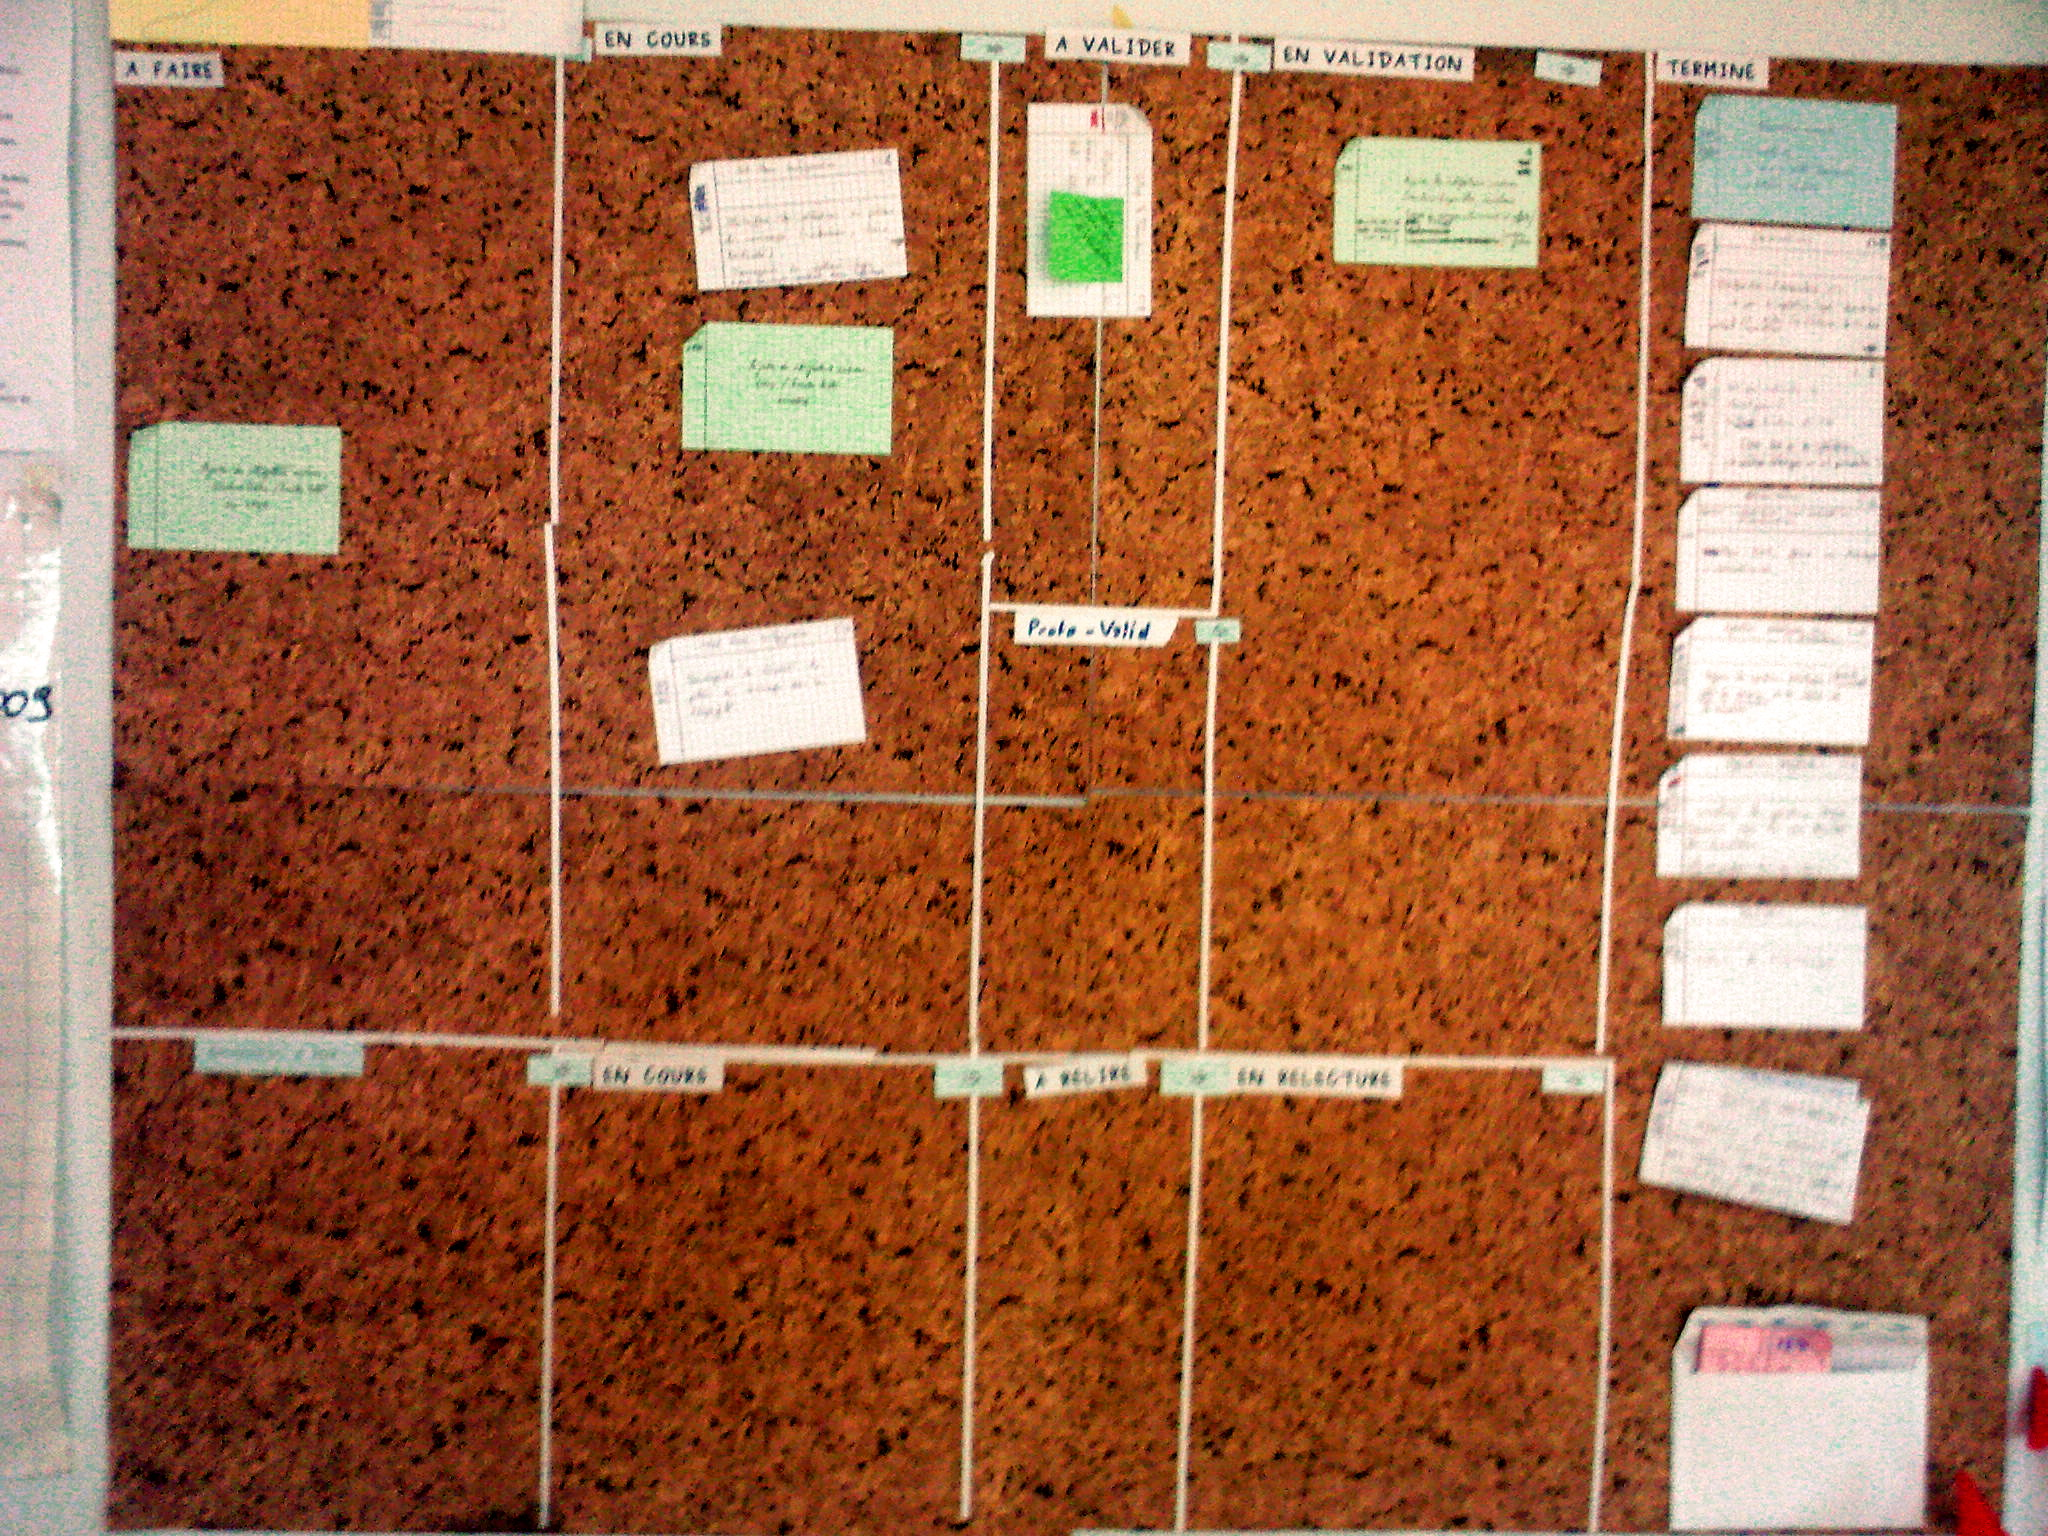
\includegraphics[width=.55\textwidth]{img/SP_A0183.jpg}
\caption{Image sample}
\label{figure:sampe}
\end{figure}

Ici du texte et du blabla, ce que l'on veut dire et écrire. A remplacer. Ici du texte et du blabla, ce que l'on veut dire et écrire. A remplacer. Ici du texte et du blabla, ce que l'on veut dire et écrire. A remplacer. Ici du texte et du blabla, ce que l'on veut dire et écrire. A remplacer. Ici du texte et du blabla, ce que l'on veut dire et écrire. A remplacer. Ici du texte et du blabla, ce que l'on veut dire et écrire. A remplacer.

\subsubsection{Titre de la sous sous section}

Exemple de tableau
\begin{table}[!ht]
	\caption{\label{tableau:evolPratXP}Evolution des pratiques XP au cours du stage}
	\begin{tabular}{|l|c|c|}
		\hline
		Pratique & Début du stage & Fin du stage\\
		\hline
		Pair programming & \tick & \tick \\
		Itération & 2 semaines & 1 semaine \\
		Intégration continue & \tick & \tick \\
		Niko Niko & \tick & \badtick \\
		Lecture & \tick & \badtick \\
		Point perso & hebdomadaire & nouvelles experimentations\\
		Pomodoro & \badtick & \tick \\
		Test driven development & \tick & \tick \\
		``Done done'' & théorique & adopté et normalisé\\
		``No Bugs'' & imprécis & engagement \\
		Slack Time & \badtick & adopté et normalisé\\
		Rétrospective & 1 à 2h le lundi matin & Timeboxée et juste après la livraison\\
		Point technique & assez réguliers & moins nombreux\\
		Veilleur & \tick & Robin cumule son rôle\\
		Batman/Robin & \badtick & \tick \\
		\hline
	\end{tabular}
\end{table}

\subsection{Conclusion}

Ici du texte et du blabla, ce que l'on veut dire et écrire. A remplacer. Ici du texte et du blabla, ce que l'on veut dire et écrire. A remplacer. Ici du texte et du blabla, ce que l'on veut dire et écrire. A remplacer. Ici du texte et du blabla, ce que l'on veut dire et écrire. A remplacer. Ici du texte et du blabla, ce que l'on veut dire et écrire. A remplacer. Ici du texte et du blabla, ce que l'on veut dire et écrire. A remplacer.

Ici du texte et du blabla, ce que l'on veut dire et écrire. A remplacer. Ici du texte et du blabla, ce que l'on veut dire et écrire. A remplacer. Ici du texte et du blabla, ce que l'on veut dire et écrire. A remplacer. Ici du texte et du blabla, ce que l'on veut dire et écrire. A remplacer. Ici du texte et du blabla, ce que l'on veut dire et écrire. A remplacer. Ici du texte et du blabla, ce que l'on veut dire et écrire. A remplacer.

\subsection{Titre de la sous section}

Ici du texte et du blabla, ce que l'on veut dire et écrire. A remplacer. Ici du texte et du blabla, ce que l'on veut dire et écrire. On peut faire une citation \cite{Motclef1}.
A remplacer. Ici du texte et du blabla, ce que l'on veut dire et écrire. A remplacer. Ici du texte et du blabla, ce que l'on veut dire et écrire. A remplacer. Ici du texte et du blabla, ce que l'on veut dire et écrire. A remplacer. Ici du texte et du blabla, ce que l'on veut dire et écrire. A remplacer.

Ici du texte et du blabla, ce que l'on veut dire et écrire. A remplacer. Ici du texte et du blabla, ce que l'on veut dire et écrire. A remplacer.
Ici du texte et du blabla, ce que l'on veut dire et écrire. A remplacer. Ici du texte et du blabla, ce que l'on veut dire et écrire. A remplacer. Ici du texte et du blabla, ce que l'on veut dire et écrire. A remplacer. Ici du texte et du blabla, ce que l'on veut dire et écrire. A remplacer.

\subsection{Titre de la sous section}

Ici du texte et du blabla, ce que l'on veut dire et écrire. A remplacer. Ici du texte et du blabla, ce que l'on veut dire et écrire. On peut faire une citation \cite{Motclef1}.
A remplacer. Ici du texte et du blabla, ce que l'on veut dire et écrire. A remplacer. Ici du texte et du blabla, ce que l'on veut dire et écrire. A remplacer. Ici du texte et du blabla, ce que l'on veut dire et écrire. A remplacer. Ici du texte et du blabla, ce que l'on veut dire et écrire. A remplacer.

Ici du texte et du blabla, ce que l'on veut dire et écrire. A remplacer. Ici du texte et du blabla, ce que l'on veut dire et écrire. A remplacer.
Ici du texte et du blabla, ce que l'on veut dire et écrire. A remplacer. Ici du texte et du blabla, ce que l'on veut dire et écrire. A remplacer. Ici du texte et du blabla, ce que l'on veut dire et écrire. A remplacer. Ici du texte et du blabla, ce que l'on veut dire et écrire. A remplacer.

\clearpage


\section{Web issues}

To understand the issues that arises when developing a web site or web application, let me first remind you how a user can access a web page.
\begin{itemize}
\item First, the client (the user's web browser) requests a web page located on a web server. The function of this web server is to deliver the requested web page to the client. This means delivery of an HTML document along with additional content, 
such as images, stylesheets and JavaScripts.
\item The client's web browser application then processes the content and displays it for the user.  
\end{itemize}

\begin{figure}[!l]
\centering
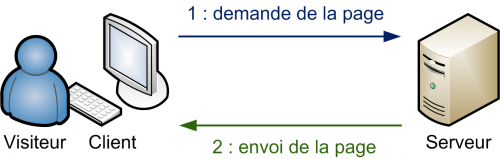
\includegraphics[width=.55\textwidth]{img/static.png}
\caption{Case of a static Html page}
\label{figure:static page}
\end{figure}
\begin{figure}[!r]
\centering
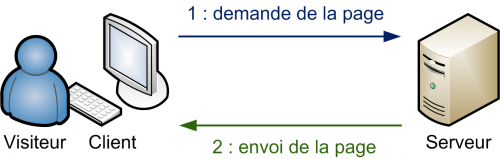
\includegraphics[width=.55\textwidth]{img/static.png}
\caption{Basic Case of a dynamic page (for example a php page)}
\label{figure:dynamic page}
\end{figure}

While the server will always deliver the same content for the same requested page, two different users might see two different things on their computer. 
The reason is that there are more than one web browser software application existing, and while they try to make it look the same, the process behind the display and interpretation of the content is not. Set aside Html content, which is quite processed in the same way among every browsers, issues arises with interpretation of
JavaScript and Stylsheets (CSS). For example, Firefox will understand the CSS property moz-border-radius while Google Chrome and Internet Explorer will not. Also, Firefox will not understand the JavaScript Object window.event while Google Chrome and Internet Explorer will. There are dozens of example like these ones.
While you can develop the server side part of the application in one language and not worry about its ability to always deliver the same content, you can't afford to develop the client side application for only one browser. This would result in many internet users not to be able to see the content as intended.
\begin{figure}[!ht]
\centering
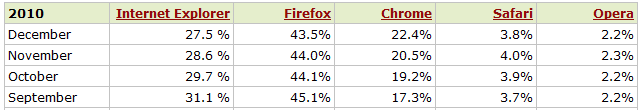
\includegraphics[width=.55\textwidth]{img/browser_statistics.png}
\caption{Basic EWS architecture }
\label{figure:Market Share of Web Browser}
\end{figure}
And as a web development company, that is even less of an option. (your clients won't like that if you tell them that only 30 of the internet users will be able to use their website.)
Web application that behaves the same way in multiple browser are called "cross-browser". 
My job was of course to make sure that every web content I created was cross-browser (at least for IE7, IE8, Chrome and FF).
At first, this can look like a hard task to accomplish, because you would need to be aware of each browser specificities. Fortunately, some tools exists to help you reach that goal.

\subsection{JavaScript}

JavaScript has some big differences between browsers. For example, to attach an event to an element, Firefox and Chrome uses the function addEventListener. Internet Explorer will not understand this function as it uses attachEvent for the same purpose. %(cf Appendix page ## http://www.quirksmode.org/dom/w3c\_CSS.html).
Also, one of the purpose of JavaScript is being able to handle all the html elements in the web page to increase the user experience on the website. And again, there are some slight differences between every browser.
Because of all those disparities, people started to build APIs, which would considerably reduce the knowledge needed of those disparities to run a cross-browser JavaScript code. On of the most famous is jQuery. Simple, yet powerful, you can find in jQuery all the JavaScript functionalities, encapsulated in cross-browser functions. Ex: instead of having to test if the browser is IE to call the function attachEvent instead of addEventListener, you can just call the jQuery method bind to attach an event to an element. No need to learn the supported functions of each browser, you just need to learn a simple API. jQuery even simplifies some JavaScript functionalities, such as the use of Ajax.
%(cf piece of code w w/o jQuery).

\subsection{CSS}

Unlike in JavaScript, there is no API to help you with CSS (mainly because CSS is not a programming language). The huge issues in CSS arises when you want to make it work on Internet explorer. Usually, you are going to develop with Chrome or Firefox (Internet Explorer can be very slow so it can be frustrating to develop on it) where the same CSS is going to work on each other. It might even work in Internet Explorer 8 (with some really little adjustment on precise cases). But most of the time, you are going to have to do some adjustments so that it works on Internet Explorer 7. Those adjustment might be to just rethink the way of styling an element so that the same CSS will work on IE7 or completely tweaking the CSS just for Internet Explorer.
The last is called "CSS hacking". And fortunately, probably because Microsoft knows that his CSS handling is not that good, it introduced what is called conditional comments. It looks like a simple html comments in the html content, but IE knows it is aimed at him and can process it to add a specific Stylesheet. Other browsers will just ignore it, as it is a mere comment for them. (cg example html + speak about prefix * \_ etc.). 
\begin{figure}[!r]
\centering
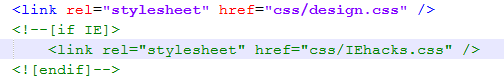
\includegraphics[width=.55\textwidth]{img/comments.png}
\caption{Basic Conditional Comment}
\label{figure:conditional comment}
\end{figure}
Another way to tweak the CSS specifically for Internet Explorer is to add a specific prefix to each CSS property you want to be applied only to some Internet Explorer Versions. (prefix * : IE 7 and below,prefix \_: IE6 and below). The downside of this is that it renders the CSS invalid to the W3C specification.

Understanding all that, you can understand why creating a site builder application is even more of a challenge. Indeed, we have to provide the user that has no understanding of html, CSS or JavaScript the ability to create a cross-browser website. And that was an important point, because it could give us an advantage against other competitors, who are not always cross-browser compliant.




\chapter{Conclusion}

\section*{Overview of the work achieved}

%During this internship I completed the realization of three add-ons (Flash Maker,
%Calendar and Carousel) as well as an administrator for current and further HTML
%add-ons.
%These add-ons were tested and approved by my tutor but in my opinion we need to
%take more time to test all configuration cases, especially since there are so many
%cases that we cannot reproduce.
%
%One thing that definitely remains to do is add more templates, more presets to these
%add-ons to provide to the user a lot more possibilities of customization and
%examples. This part concerns more the designers that need to imagine and create
%templates and a small intervention from developer to integrate these.
%
%We are also expecting to launch last version of Easy Web Content containing all new
%add-ons soon so we can have feedback from users.
%
%We also have a lot of ideas for new add-ons that should be easier to create since we
%now have all required bases.
%
%I am now staying at Hindsite six other months to go on with this project, form next
%interns to this system and manage all further developments in this project.
%
%As Easy Web Content is not live at the moment I’m writing these lines we do not
%have an idea of the revenues generated through my work but I already know that
%when next version will be launched we will propose users two different subscriptions:
%- Standard account type will grant access to already existing functionalities of
%Easy Web
%- A new “Complete” account will give a full almost unlimited access to all add-
%ons to the user
%
%This Complete account will be proposed at a price of \$24.95 a month whereas
%standard account is at \$9.95.
%As the Complete account added value is important we hope to generate good
%revenues from this subscription and expect many users to switch to this account.

\section*{Work and organization}

%I feel like my work was really useful because I could see the results of it.
%In the United States the hours of work per week are greater than in France (around
%40 hours) and I was mostly satisfied with the progression of my work.
%I was granted a lot of independency in the choice of technologies, implementation,
%methods and organization. I could always give my opinion and submit my ideas.
%In the other hand I think that we can still improve a lot the organization of the work at
%Hindsite.
%
%For example we do not have any Subversion (CVS) to work with and as we were at
%least two people working on shared resources this was always a pain to work with
%and it happen that we lose time because of that.
%This is a point that me and previous interns already talked about to Mr. Taei but
%because do not have access to the server configuration we cannot configure a SVN
%ourselves.
%
%Another improvement of organization would be to use a Bug Tracker tool; we are still
%working with shared documents to track bugs.

% Pour finir l'interligne de 1,5
\end{onehalfspace}

%----------------------------------------
% Pour la bibliographie
%----------------------------------------
% Citer tous les ouvrages/références
% pour ajouter des references : ouvrir biblio.bib
%nocite permet d'ajouter de la biblio sans avoir aciter 
%quelquechose dans le document
% si quelquechose a citer voir \cite
\nocite{MotClef1}
\nocite{MotClef2}
\nocite{MotClef3}
\nocite{MotClef4}
\nocite{MotClef5}
% Trier par ordre d'apparition
%bibliographystyle{unsrt}
% Pour le style de la biblio
\bibliographystyle{plain}
\bibliography{biblio}
\printindex
%exemples d'annexes
\appendix
\chapter{Site Builder Competitors}\label{annexe:ews-competitors}
\begin{figure}[!ht]
\centering
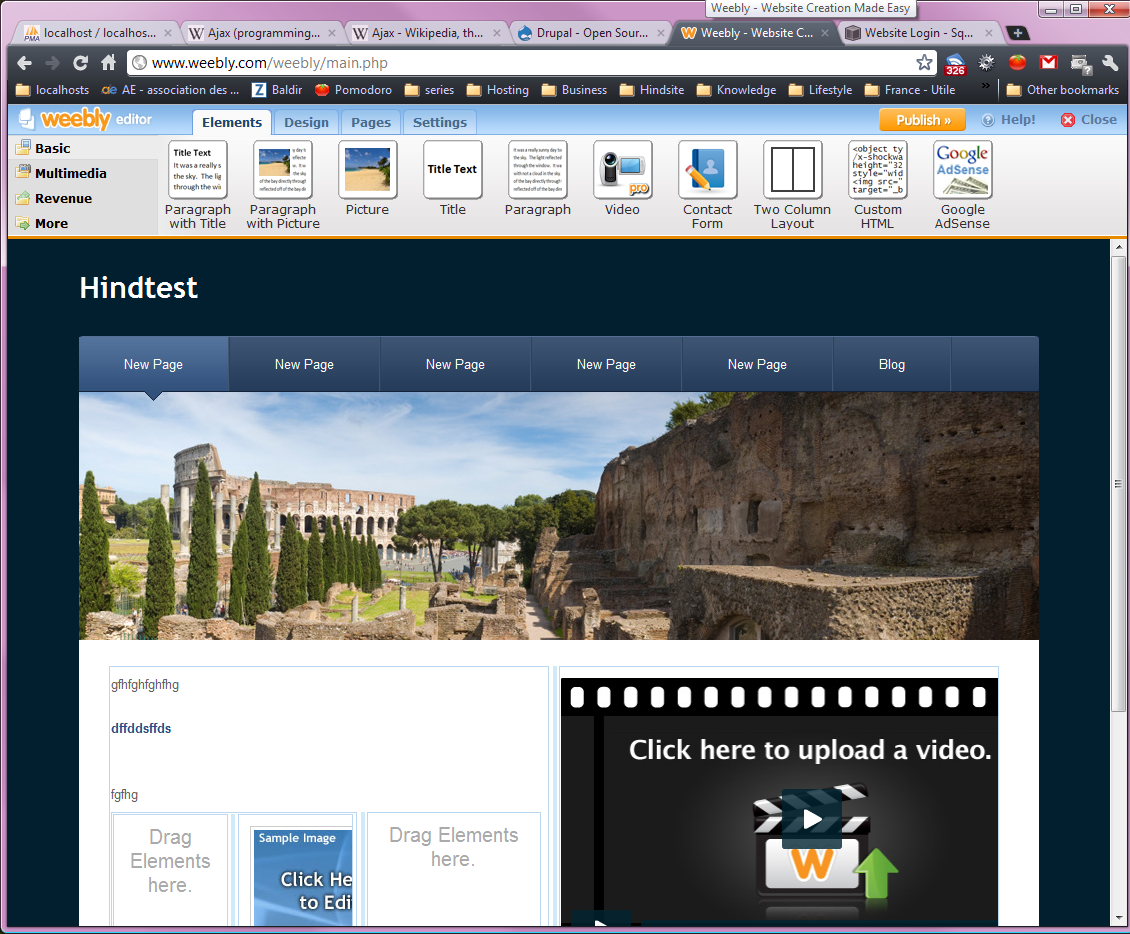
\includegraphics[width=.70\textwidth]{img/weebly.png}
\caption{Weebly}
\label{figure:weebly}
\end{figure}

\begin{figure}[!ht]
\centering
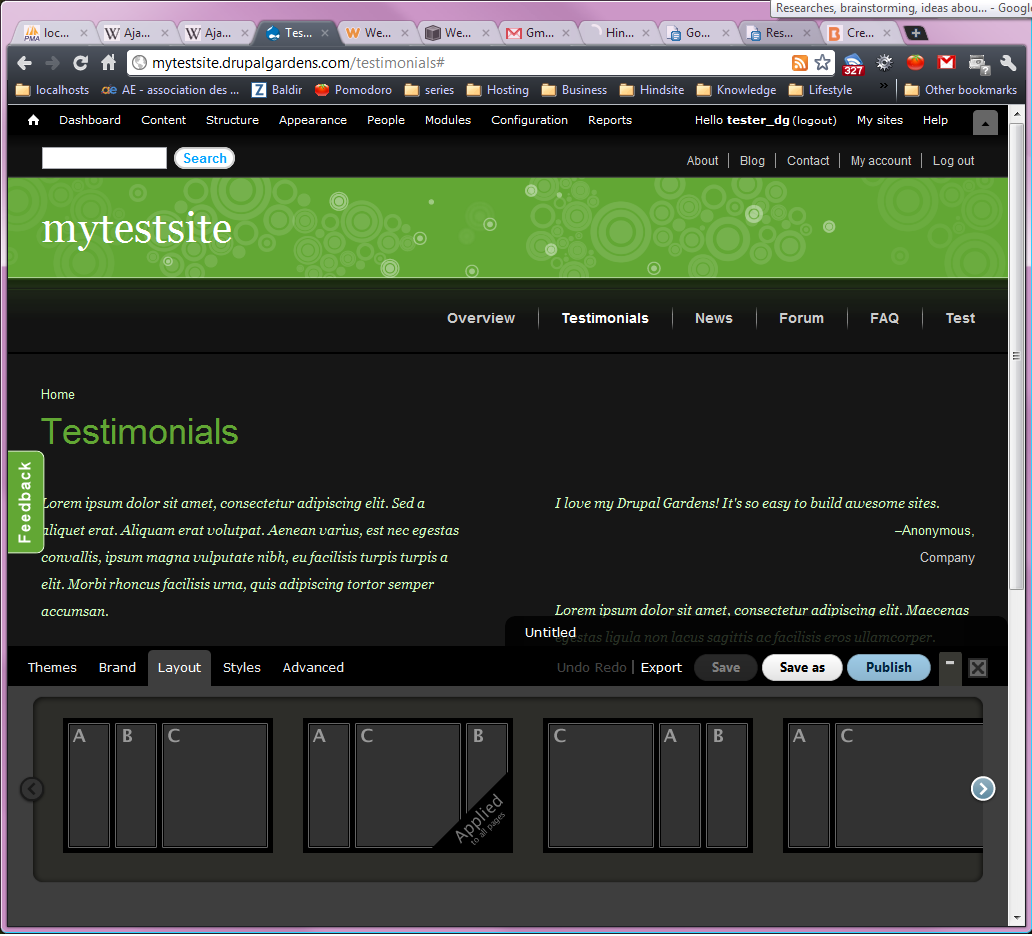
\includegraphics[width=.70\textwidth]{img/drupal_gardens.png}
\caption{Drupal Gardens}
\label{figure:drupal_gardens}
\end{figure}

\begin{figure}[!ht]
\centering
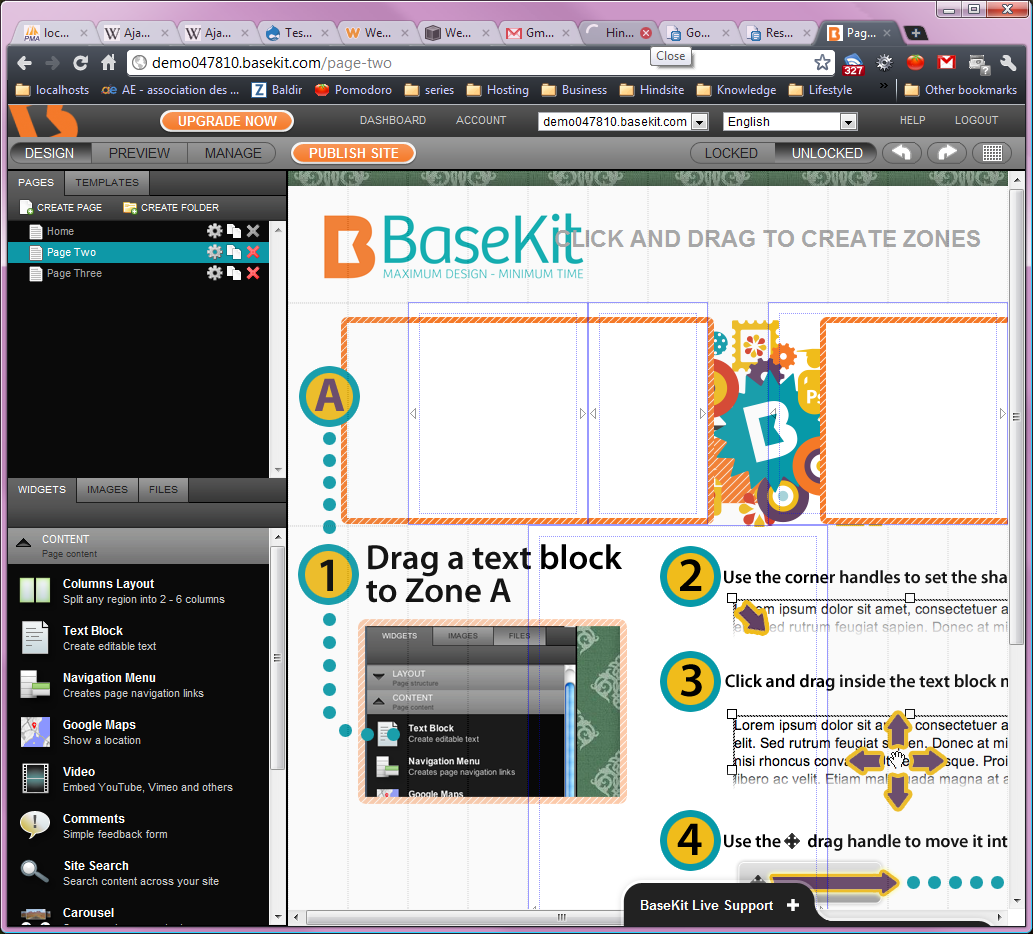
\includegraphics[width=.70\textwidth]{img/basekit.png}
\caption{BaseKit}
\label{figure:basekit}
\end{figure}

\begin{figure}[!ht]
\centering
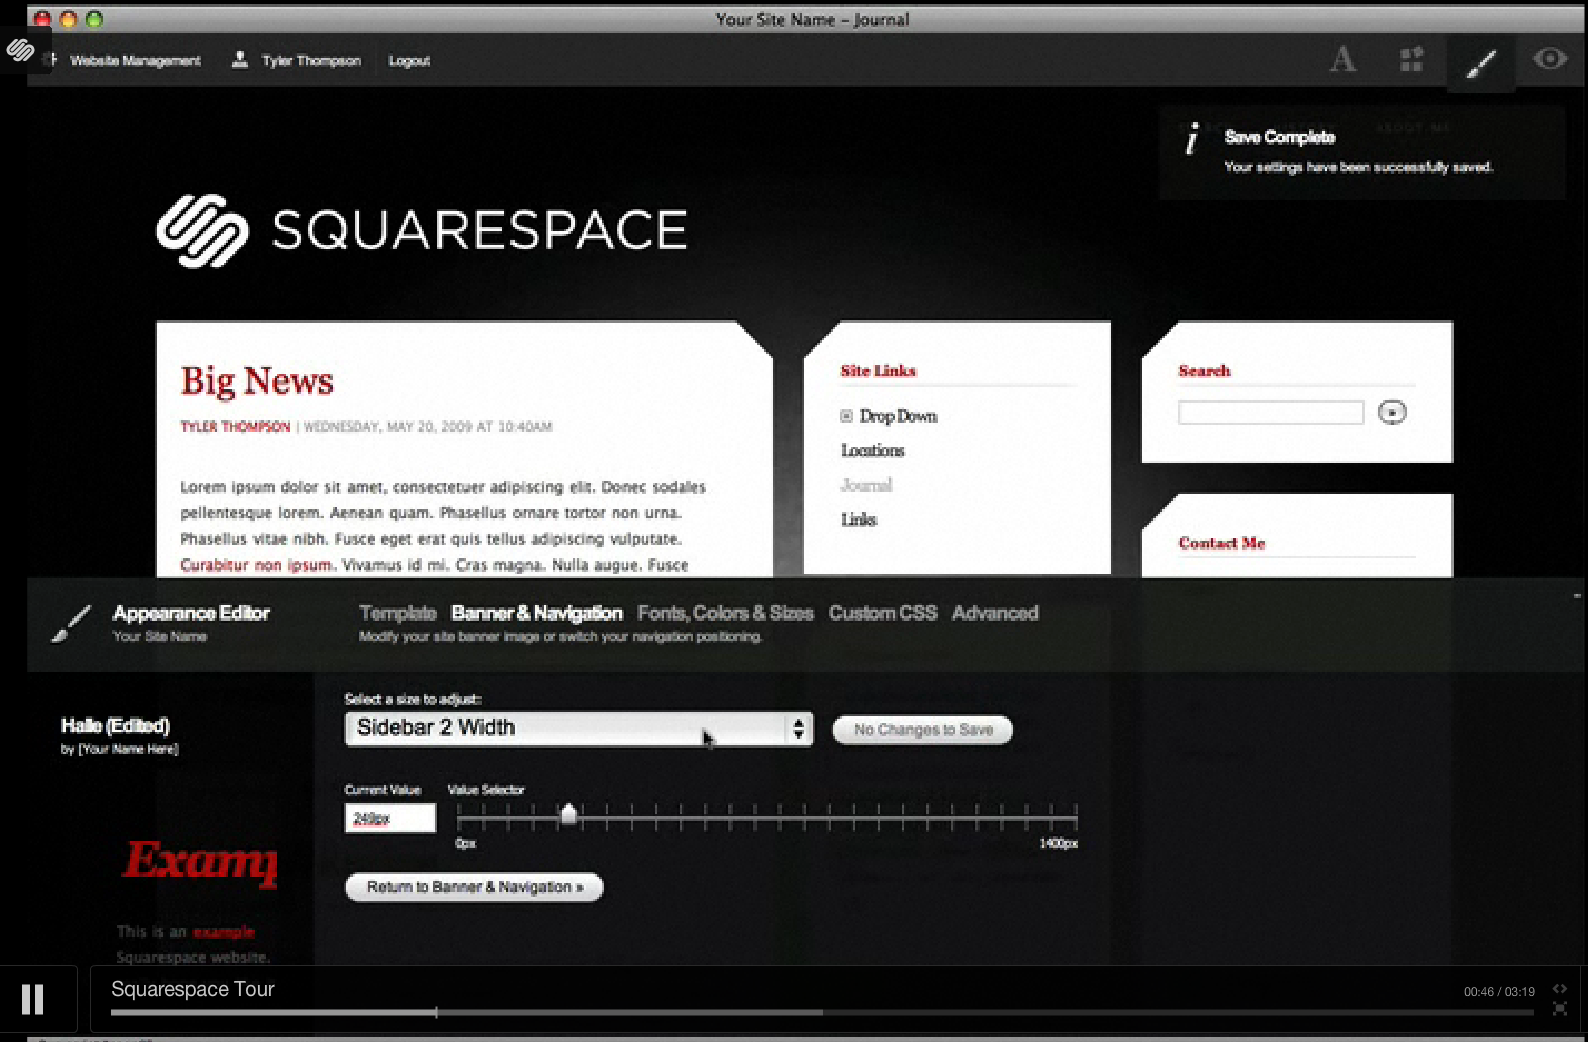
\includegraphics[width=.70\textwidth]{img/squarespace.png}
\caption{Squarespace}
\label{figure:squarespace}
\end{figure}
\chapter{Cross browser issues}\label{annexe:JavaScript differences}


\section*{Example of javascript differences between browsers}
\begin{figure}[!ht]
\centering
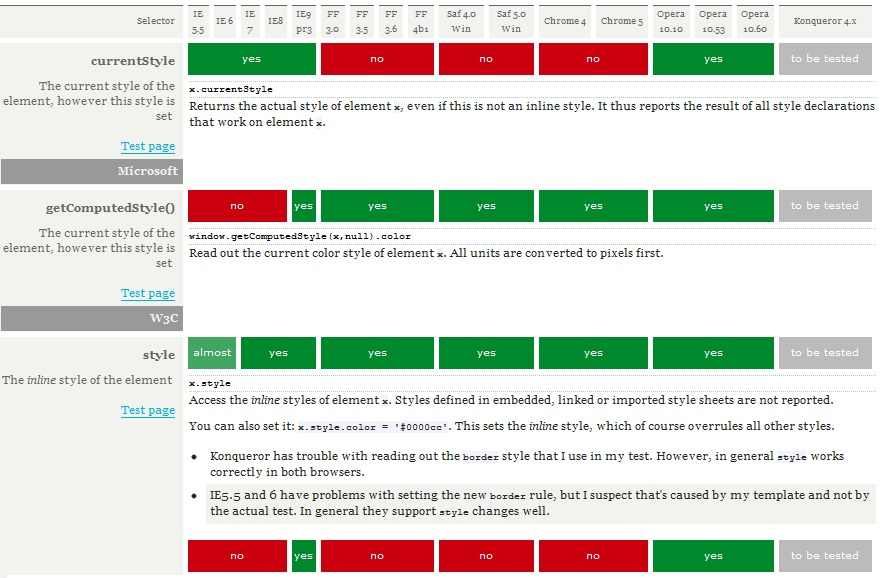
\includegraphics[width=\textwidth]{img/css.jpg}
\caption{Css handling differences}
\label{figure:market-brosers}
\end{figure}


\chapter{Pomodoro Technique}\label{annexe:pomodoro}

\paragraph*{Qu'est ce que c'est?}La technique du pomodoro a été inventée par Fransesco Cirillo. C'est une technique de gestion du temps qui peut être utilisée pour n'importe quelle type de tâche. L'objectif de la technique du pomodoro est de considérer le temps comme un allié dans ce que l'on veut faire et d'améliorer en permanence notre façon de travailler ou d'étudier.

\paragraph*{Que faut-il pour commencer?}
\subparagraph*{Une minuterie de cuisine}
Vous pouvez aussi bien utiliser un pomodoro\footnote{minuterie de cuisine} qu'un timer logiciel. Le régler sur 25 minutes.


% 4eme de couverture
%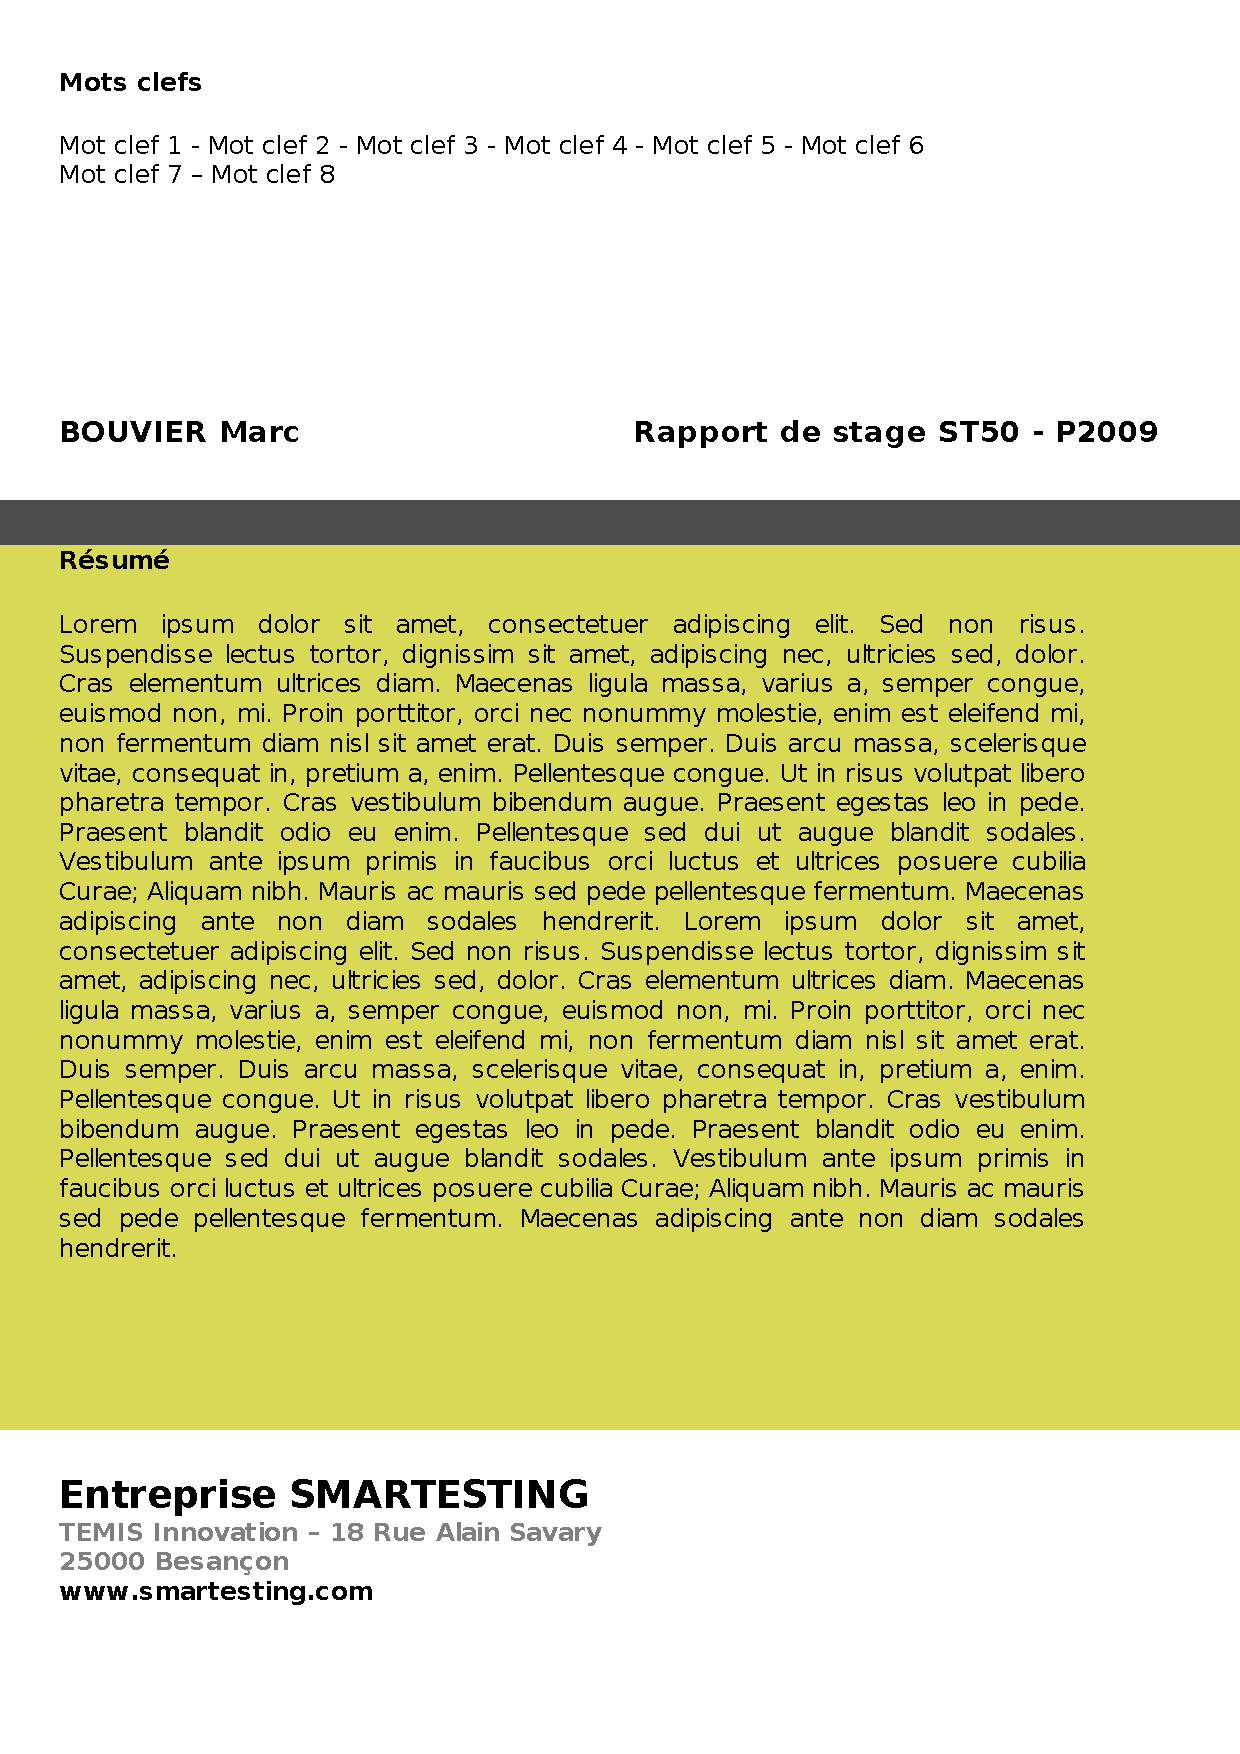
\includepdf[pages=1,noautoscale=false]{derniere_page.pdf}
\end{document}
